%!TEX root = ../thesis.tex
% chapter 4

\chapter{Charge and energy confinement}
\label{sec:ch4}

Most SCP research has been conducted without considering medium inhomogeneity due to theoretical and experimental challenges. Nonetheless, there is a good possibility that an SCP will be produced in an inhomogeneous medium containing mesoscopic particles. For example, instantaneous cooling and local condensation in the planet's atmosphere caused by storms, followed by lightning, or unavoidable flaws in the manufacture of targets for the inertial confinement fusion \cite{clark2010plastic, wang2017development}. These facts lead us to wonder what impact the medium's inhomogeneity and mesoscopic particles have on SCPs.

We use a nanosecond pulse laser to generate an SCP on the quasi-equilibrium phase coexisting supercritical fluid that we discovered in our previous research (Chap.\ref{sec:ch2}) to examine the influence of medium inhomogeneity on the charge and energy transport of SCPs. In contrast to the textbook definition, the supercritical fluid has been observed to have more liquid or gas-like characteristics rather than being a homogenous and structureless single-phase \cite{simeoni2010widom, gorelli2006liquidlike, banuti2015crossing, maxim2019visualization, pipich2018densification, pipich2020polymorphic, prescher2017experimental, proctor2018liquid, bryk2017behavior, ploetz2019gas, schienbein2018investigation}. In addition, we discovered that the submicron-sized liquid-like fluid packages survive in the supercritical environment for an unusually long duration.

According to our findings, inhomogeneity and mesoscopic particles in such a medium improve the charge and energy confinement of SCPs. This finding suggests that the medium state has a significant impact on the transport of SCPs with similar coupling characteristics.



%----------------------------------------------------------------------------------------------------
\section{Experimental apparatus and conditions}
\label{sec:ch4-1}

In the process of increasing the chamber pressure up to $100 \text{ bar}$ by controlled compression-expansion cycles of argon fluid, large populations of liquid-like fluid packages ranging in size from several nanometers to sub-micrometer are created. The coexistence of liquid-like mesoscopic particles in the supercritical fluid causes the inhomogeneity of the medium preserves for an hour timescale. After 2 hours, the liquid-like particles dissolve, and the medium becomes homogeneous. The irradiation of high-intensity nanosecond laser pulse into a dense and (in)homogeneous medium produces the elongated plasma jets. The Fig.\ref{fig:290gen} through \ref{fig:700ext}) show the filtered images of the plasma jets. While broadcasting the structural features of each image, to emphasize the discrepancy in the intensities for different medium conditions, the images are relatively normalized at each time frame. Thus, a pair of plasma images both for the inhomogeneous and homogeneous medium at a certain time frame is normalized at once and by itself, not affecting other images in different time frames.

\begin{figure}[ht!]
\centering
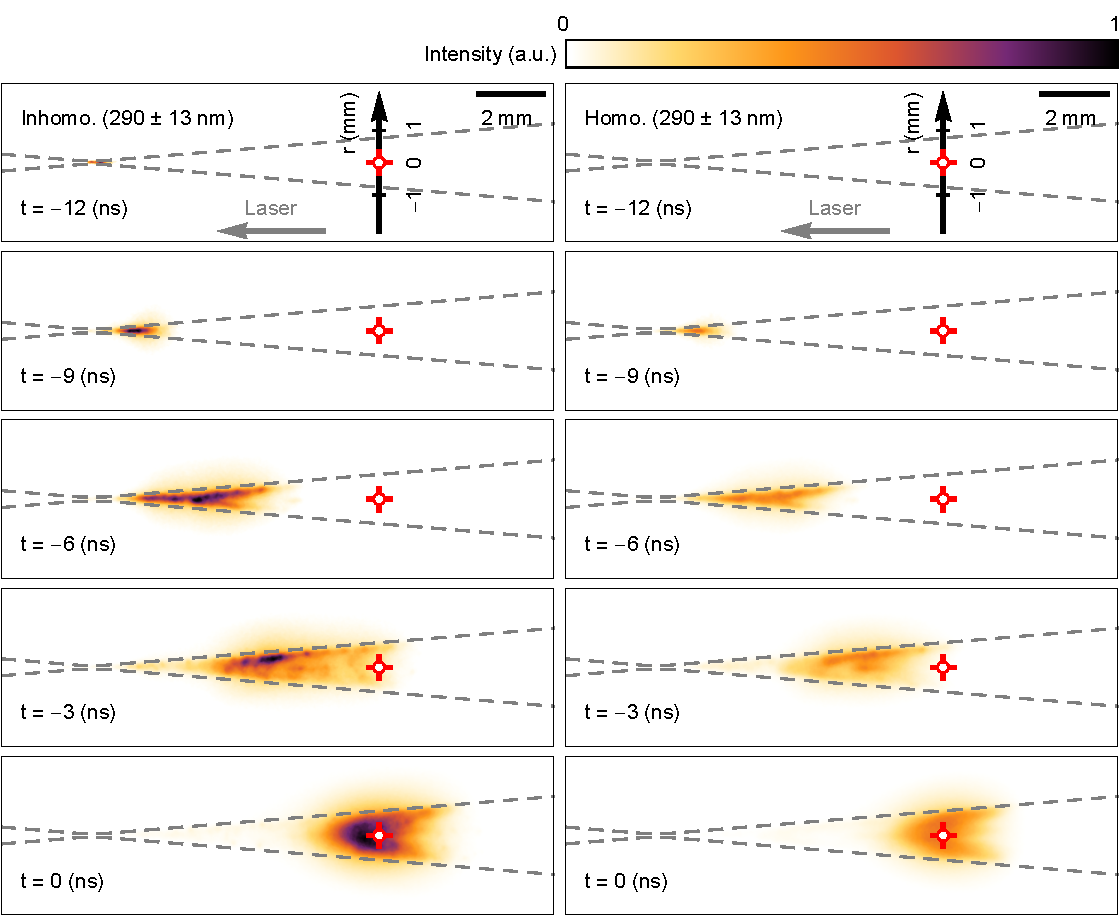
\includegraphics[width=130mm]{figures/ch4/imaging/290gen.pdf}
\caption{$290\pm13 \text{ nm}$ filtered images of the plasma discharge for the generation phase. The two columns show the plasmas in the inhomogeneous and homogeneous medium, respectively.}
\label{fig:290gen}
\end{figure}

\begin{figure}[ht!]
\centering
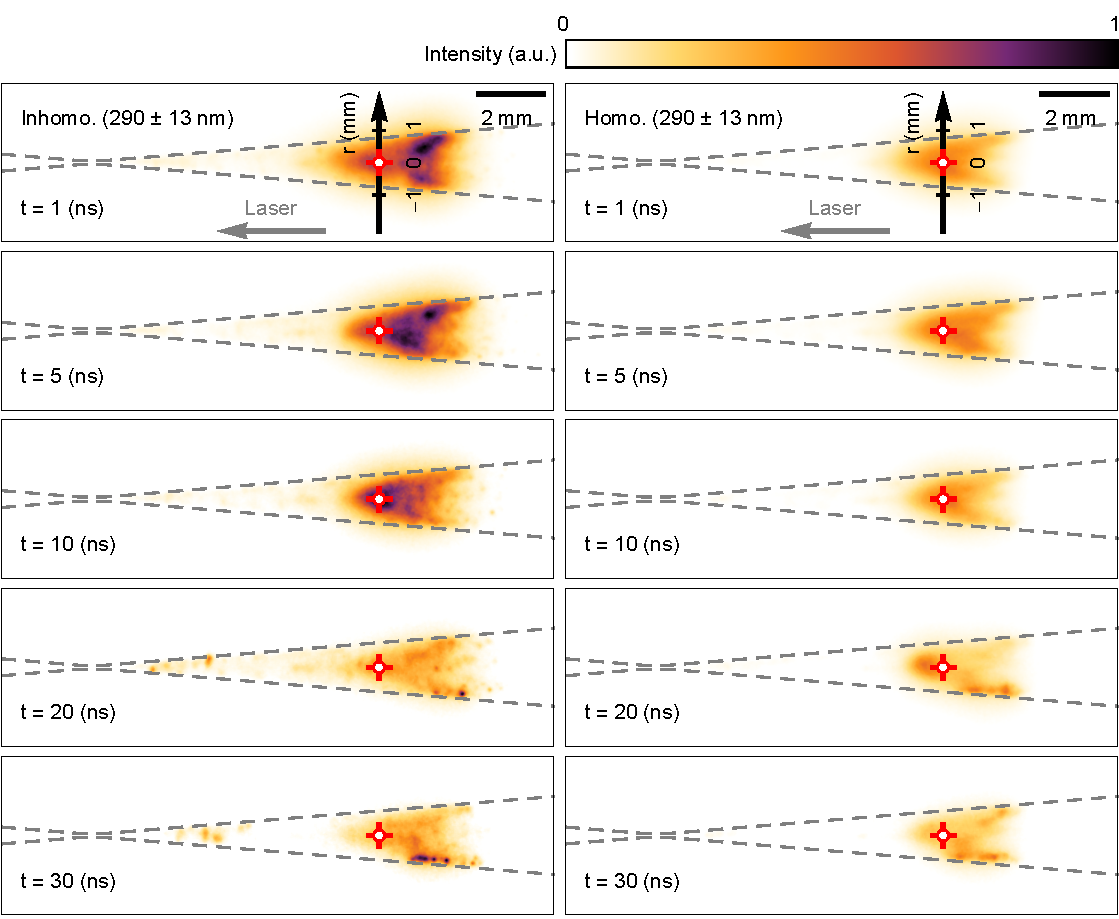
\includegraphics[width=130mm]{figures/ch4/imaging/290SCP.pdf}
\caption{$290\pm13 \text{ nm}$ filtered images of the plasma discharge for the SCP phase. The two columns show the plasmas in the inhomogeneous and homogeneous medium, respectively.}
\label{fig:290SCP}
\end{figure}

\begin{figure}[ht!]
\centering
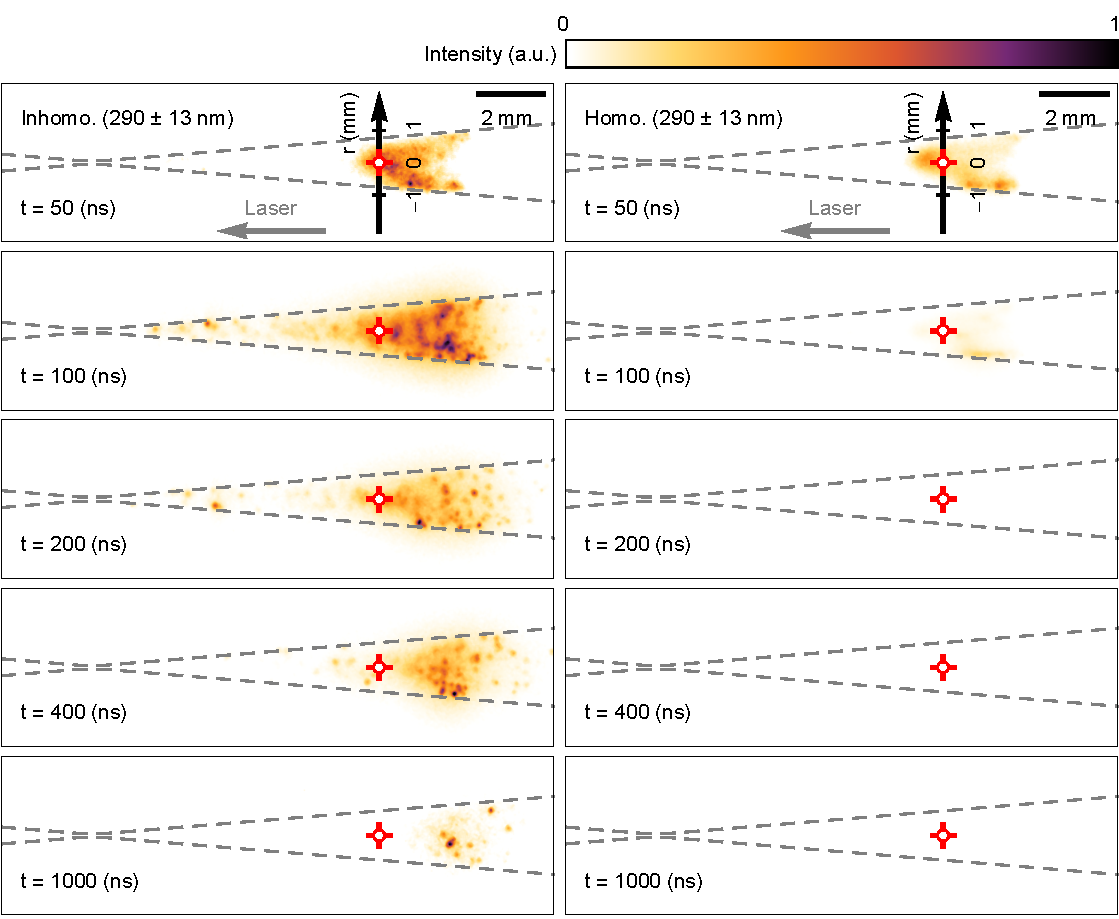
\includegraphics[width=130mm]{figures/ch4/imaging/290ext.pdf}
\caption{$290\pm13 \text{ nm}$ filtered images of the plasma discharge for the extinction phase. The two columns show the plasmas in the inhomogeneous and homogeneous medium, respectively.}
\label{fig:290ext0ext}
\end{figure}

\begin{figure}[ht!]
\centering
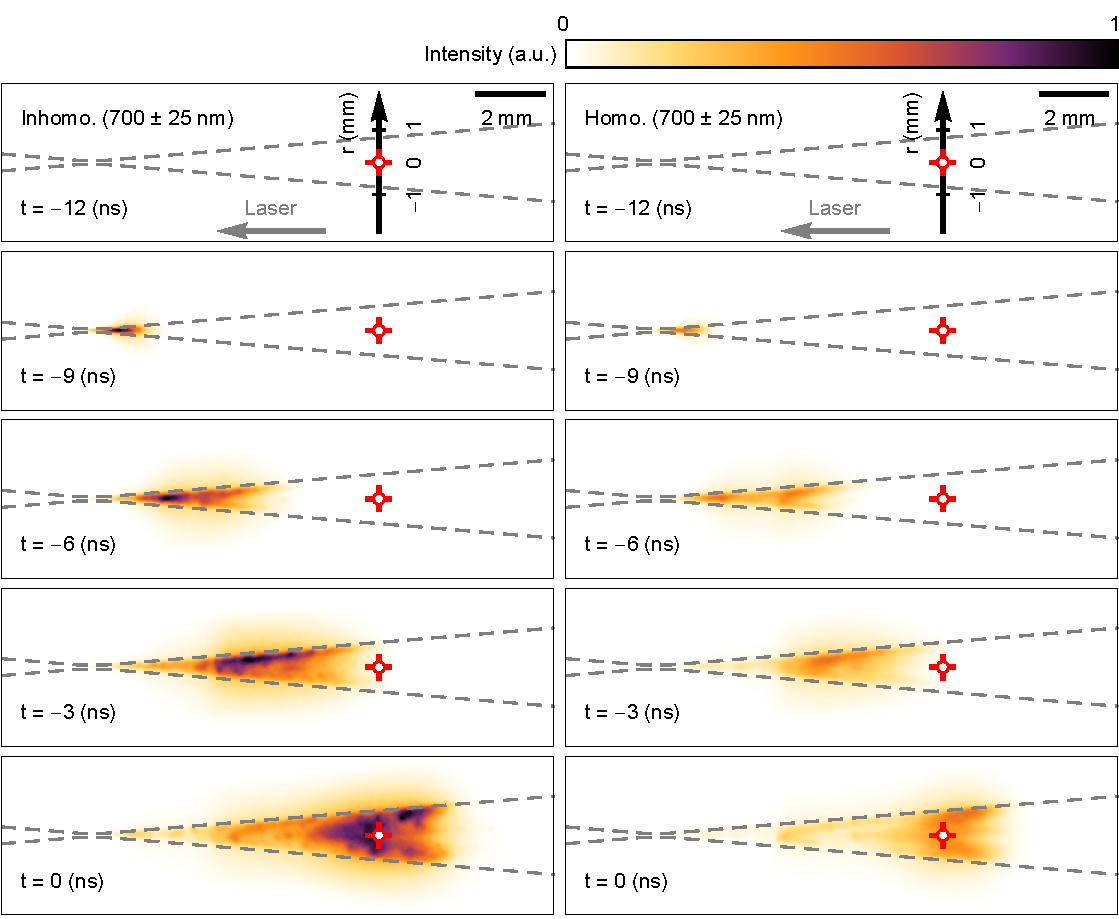
\includegraphics[width=130mm]{figures/ch4/imaging/700gen.pdf}
\caption{$700\pm25 \text{ nm}$ filtered images of the plasma discharge for the generation phase. The two columns show the plasmas in the inhomogeneous and homogeneous medium, respectively.}
\label{fig:700gen}
\end{figure}

\begin{figure}[ht!]
\centering
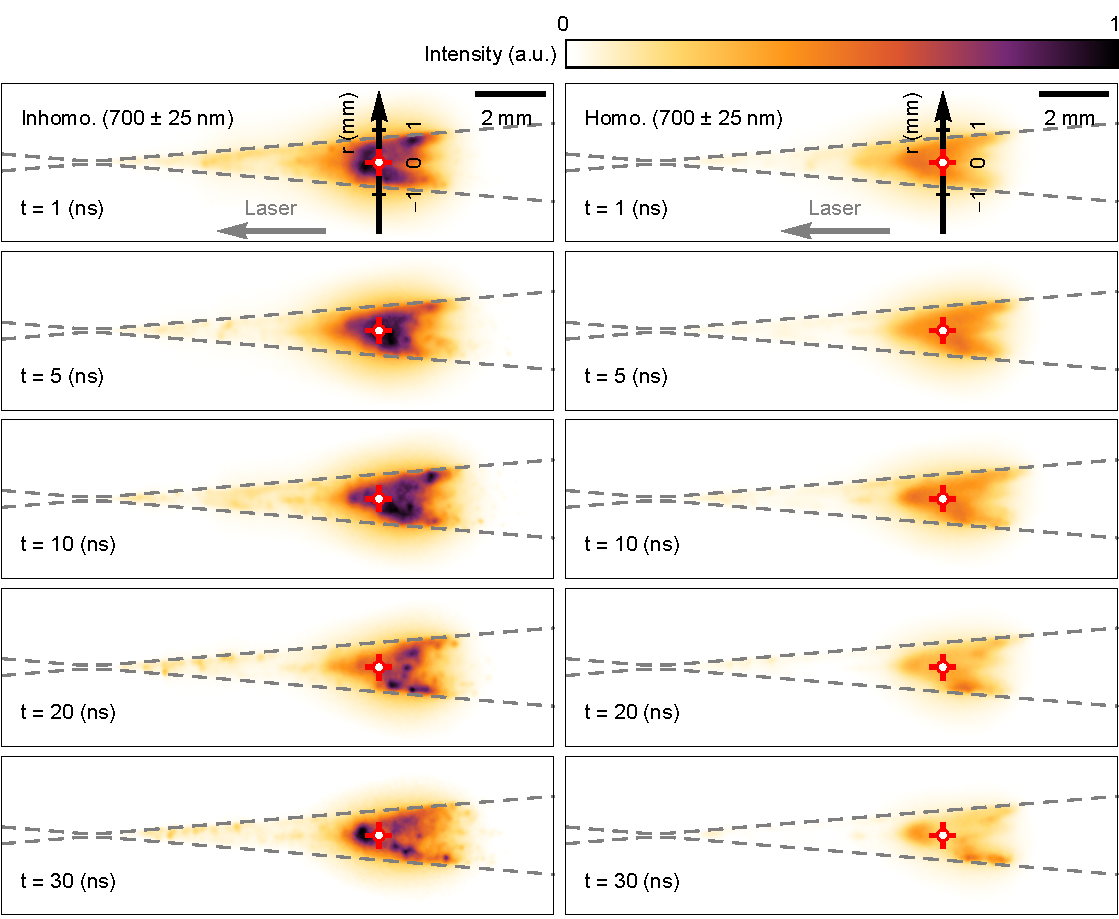
\includegraphics[width=130mm]{figures/ch4/imaging/700SCP.pdf}
\caption{$700\pm25 \text{ nm}$ filtered images of the plasma discharge for the SCP phase. The two columns show the plasmas in the inhomogeneous and homogeneous medium, respectively.}
\label{fig:700SCP}
\end{figure}

\begin{figure}[ht!]
\centering
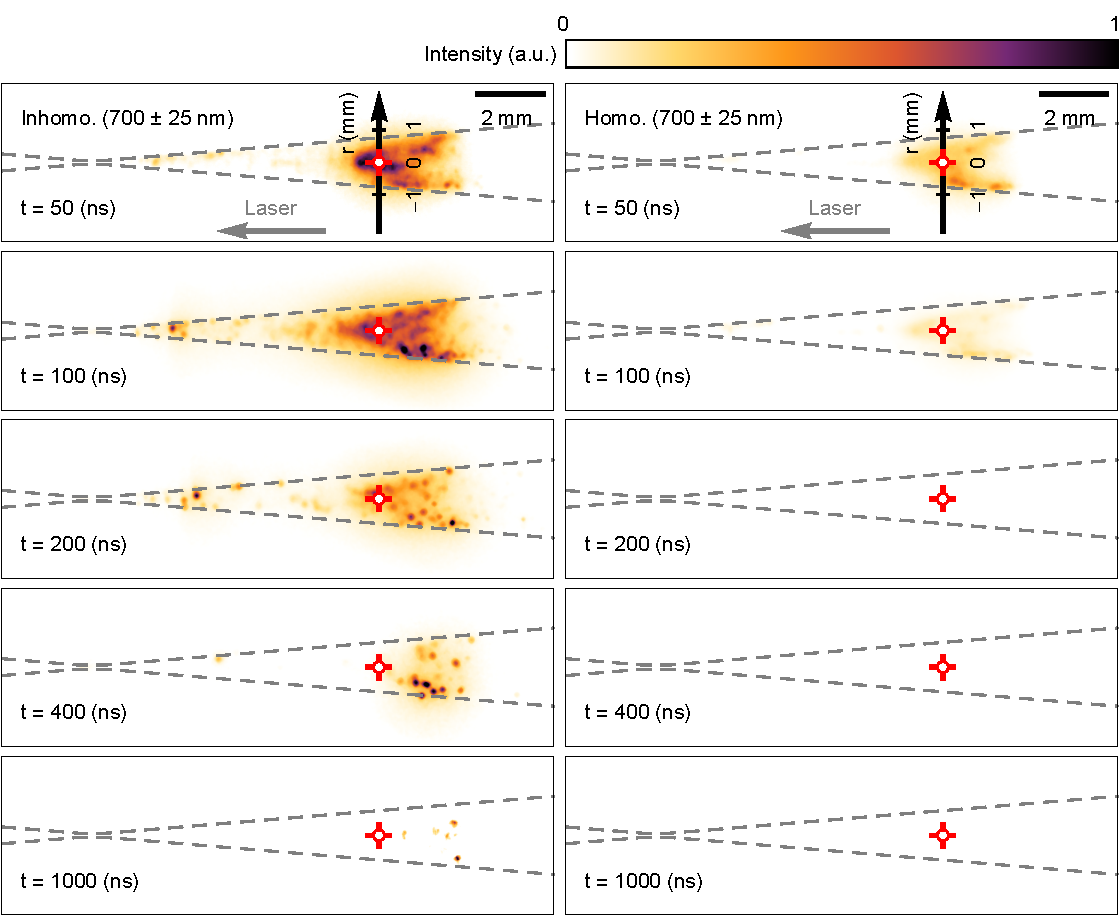
\includegraphics[width=130mm]{figures/ch4/imaging/700ext.pdf}
\caption{$700\pm25 \text{ nm}$ filtered images of the plasma discharge for the extinction phase. The two columns show the plasmas in the inhomogeneous and homogeneous medium, respectively.}
\label{fig:700ext}
\end{figure}

The SCP is generated using an Nd:YAG pulse laser (Quantel) –  wavelength: $1064 \text{ nm}$, pulse energy: $720 \text{ mJ/pulse}$, duration: $6 \text{ ns}$, and operation frequency: $2 \text{ Hz}$. The laser is focused with a $50 \text{ mm}$ AR coated plano-convex lens (Thorlabs) into the high-pressure chamber. The beam waist is about $50 ~\mathrm{\mu}\text{m}$ and the corresponding laser intensity is about $1.5 \times 10^{12} \text{ W}\cdot\text{cm}^{-2}$. The cube-shaped stainless steel chamber has five optical viewports made by a sapphire window and stainless steel housing (Rayotek). The light emission from the plasma is guided by a lens and an optical fiber (Thorlabs) to the $150 \text{ mm}$ Czerny-Tuner type monochromator (Princeton Instruments) and ICCD (Princeton Instruments) for measuring spectrum or the lens optics and ICCD for taking the images. The gate width of ICCD is manipulated from $3$ to $200 \text{ ns}$ with respect to the time delay (see the details in Appendix.\ref{sec:ap4}). Each spectrum is averaged over 50 plasma discharges to improve the signal-to-noise ratio while each image is taken from the single pulse experiment. The pulse laser is very stable, and the shot-to-shot fluctuation of the plasma emission is less than $20\%$. The spectral response of the measurement system is absolute-calibrated by using a standard light source within $10\%$ of errors (Ocean Optics). The filtered image of plasma discharge is taken separately with the ICCD. All the images presented in this work are single-shot images without averaging, and the gate widths of the ICCD are matched with the spectral data.



%----------------------------------------------------------------------------------------------------
\section{Discharge Characteristics}
\label{sec:ch4-2}

The plasma lifetime is classified into three different phases -- \textcircled{\raisebox{-0.9pt}{1}} generation phase ($-15 \sim 0 \text{ ns}$), \textcircled{\raisebox{-0.9pt}{2}} SCP phase ($0 \sim 50 \text{ ns}$), and \textcircled{\raisebox{-0.9pt}{3}} distinction phase ($50 \text{ ns} \sim$). For each phases, the images are taken with two different bandpass filters: $290\pm13 \text{ nm}$ and $700\pm25 \text{ nm}$.

In the generation phase ($-15 \sim 0 \text{ ns}$), the plasma discharge is fired near the laser focus and grows toward the laser upstream (Fig.\ref{fig:290gen} and \ref{fig:700gen}). Note that the half-width of the laser pulse is about $6 \text{ ns}$ and a spherule plasma continuously absorbs the laser pulse energy. The time zero is decided when the plasma expansion ceases and the emission intensity becomes maximum. The average expansion speed is about $1,000 \text{ km s}^{-1}$ which is much faster than any particle diffusion. Thereby, the expansion is likely due to the continuation of the Bremsstrahlung emission and inverse Bremsstrahlung absorption of photons during the collisions between electrons and ions \cite{bataller2016observation}. Although there is no preferred direction of the Bremsstrahlung process, the pre-ionization by laser pulse determines the expansion direction (see Fig.\ref{fig:ionizationWave}). The laser pulse pre-ionizes the medium as it travels to the focal point, and when it reaches the high-density plasma already generated by the pulse front, it does not proceed any further and is reflected. Therefore, pre-ionization is dominant in the laser upstream direction.

\begin{figure}[ht!]
\centering
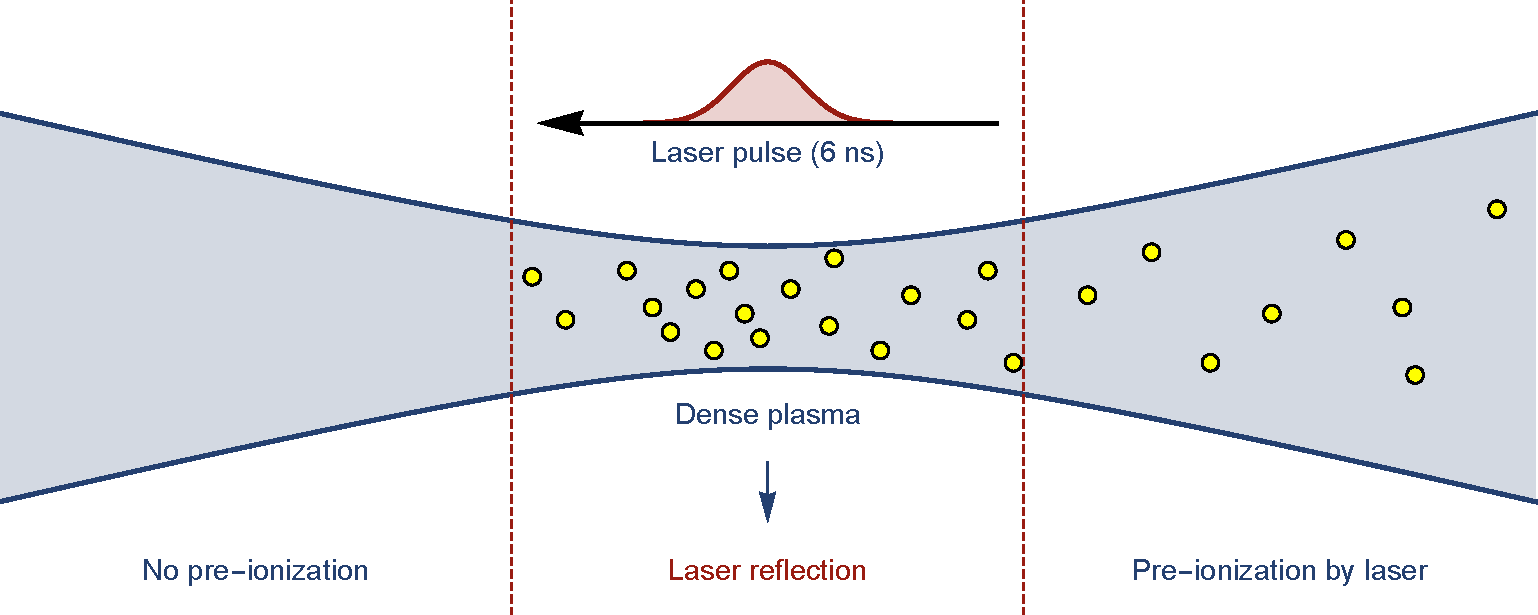
\includegraphics[width=130mm]{figures/ch4/ionization/ionizationWave.pdf}
\caption{Schematic diagram for asymmetric plasma expansion process. The incident laser pulse pre-ionizes the medium and is reflected back from the dense plasma generated at the focus of the laser itself. The spatially asymmetric pre-ionization results in asymmetric plasma expansion.}
\label{fig:ionizationWave}
\end{figure}

In the SCP phase ($0 \sim 50 \text{ ns}$), the strongly coupled condition is achieved for both plasmas in the homogeneous and inhomogeneous medium (Fig.\ref{fig:290SCP} and \ref{fig:700SCP}). For both cases, the size and structural features of plasma bulk are not distinguishable from each other in the relatively normalized images. However, the total emission intensity from the plasma in the inhomogeneous supercritical fluid is greater than that from the homogeneous medium. At this stage, the continuum radiation is dominant over the line emissions, and the plasma can be approximated as a blackbody (Fig.\ref{fig:blackbodyFit}). Further details related to the spectrum will be discussed shortly.

In the extinction phase ($50 \text{ ns} \sim$), while the volume shrinks, the plasma becomes diluted, and the line emission turns significant over the continuum radiation (Fig.\ref{fig:blackbodyFit}). The emission lasts for a longer timescale in the plasma generated in the inhomogeneous medium than in the homogeneous medium. For the inhomogeneous case, the light emission tends to illuminate from several localized points, which are the mesoscopic fluid packages in the medium. It shows that the liquid-like particles in the plasma function as the recombination sites because the atomic line emissions are mostly followed after the recombination of electrons and ions. Thereby, it implies that, during the earlier plasma phase (i.e., the SCP phase), the particles submerged in SCP store a considerable amount of electrons and serve as the charge reservoirs. It can be understood by an analogy to the charging of a refractory particle in a dusty plasma (Chap.17 in \cite{bellan2008fundamentals}). It should be pointed out that the whole story of the conventional theory of dusty plasma is only applicable for a dilute case when the Debye length is much larger than the dust size. Nevertheless, at least, the derivation of dust charging based on the unequal charge current of electrons and ions at the dust surface is still relevant as there is no need for such an assumption.



%----------------------------------------------------------------------------------------------------
\section{Plasma properties}
\label{sec:ch4-3}

\begin{figure}[ht!]
\centering
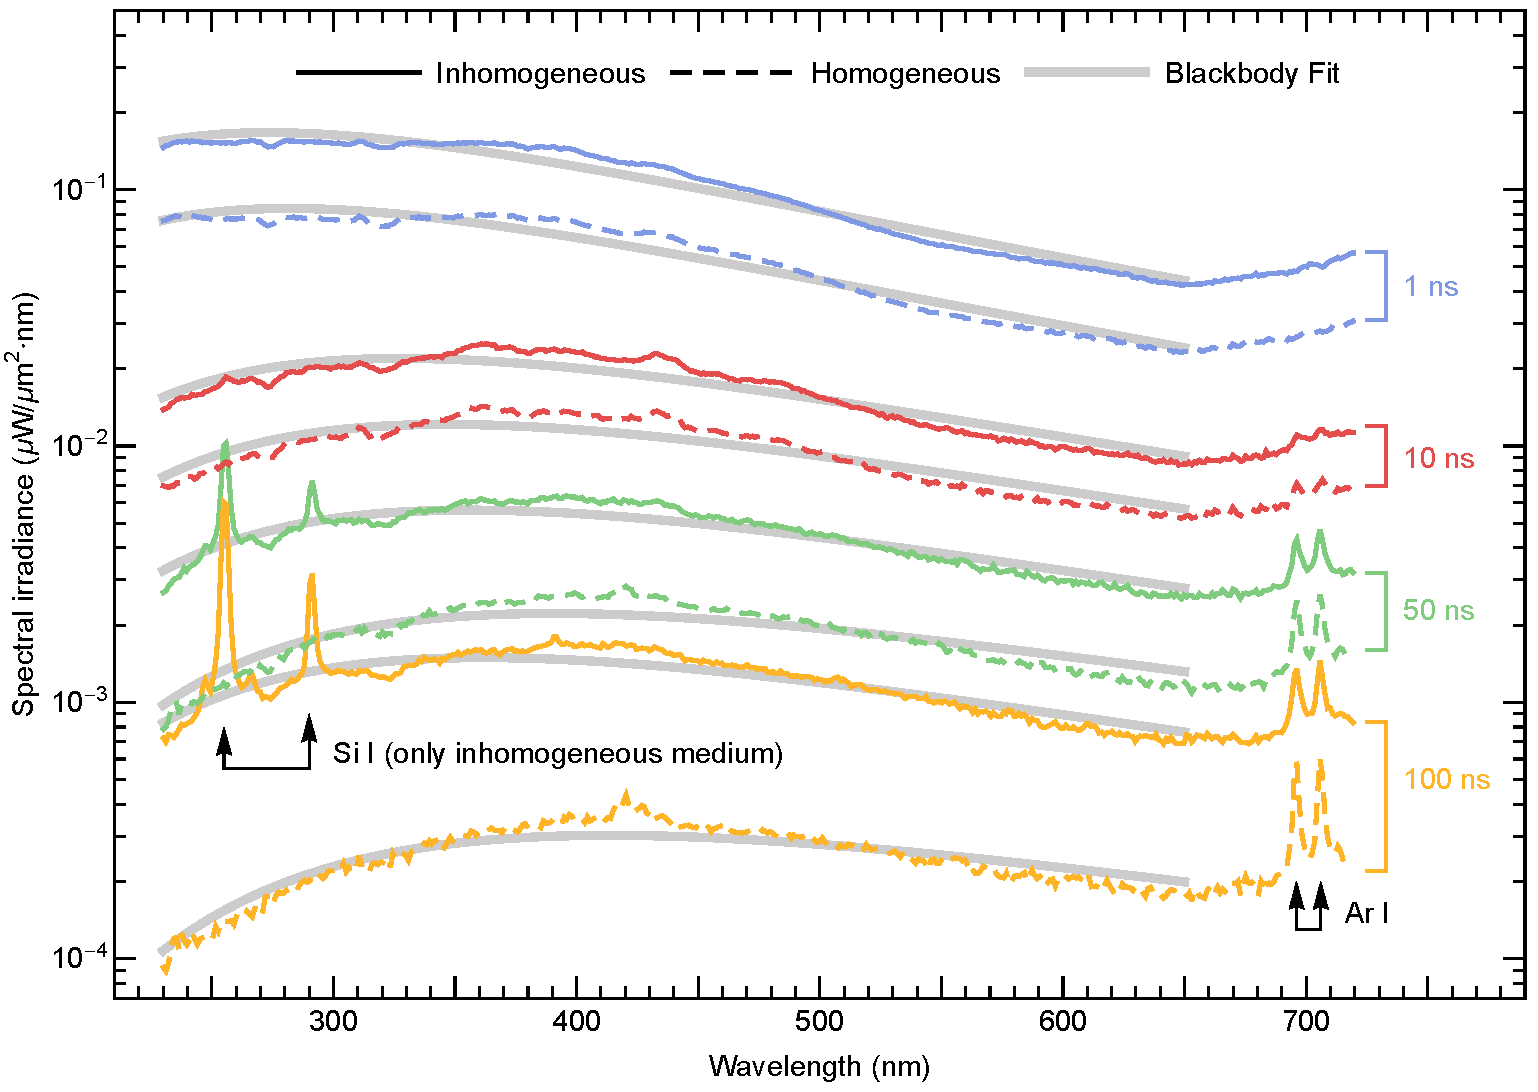
\includegraphics[width=130mm]{figures/ch4/blackbody/fit.pdf}
\caption{Absolute-calibrated broadband spectra from the SCP, and the blackbody model fits. The spectrum well fits with the blackbody radiation model in the early time when the emission is mostly continuum, and the line emission gradually increases. Only when the medium is the inhomogeneous state, the Si I peaks are observed, while the Ar I peaks appear for both cases. The deviation of relative intensity for the different medium conditions increases as time goes.}
\label{fig:blackbodyFit}
\end{figure}

\begin{figure}[ht!]
\centering
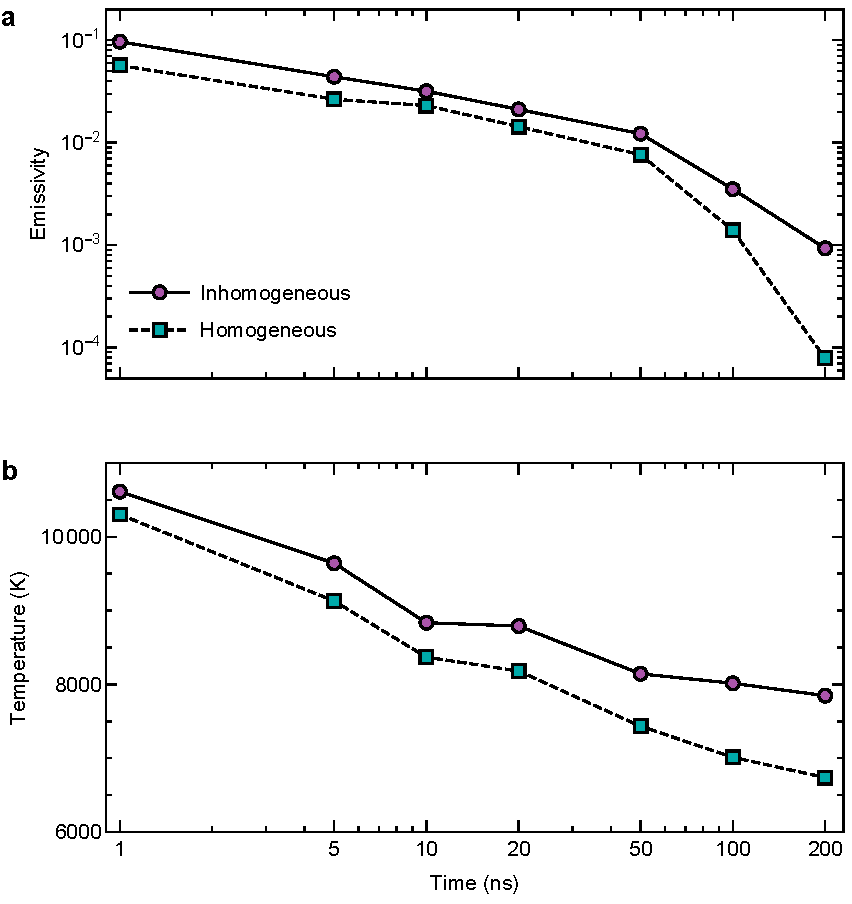
\includegraphics[width=100mm]{figures/ch4/blackbody/temporal.pdf}
\caption{The emissivity and temperature by time from the blackbody analysis of the plasma emission spectrum. Both the emissivity and temperature are higher for the plasmas in the inhomogeneous supercritical fluid. As the intensity of an ideal blackbody is proportional to the fourth power of the temperature, the higher emissivity of the plasma with a higher temperature implies much greater radiation intensity.}
\label{fig:blackbodyTemporal}
\end{figure}

\begin{figure}[ht!]
\centering
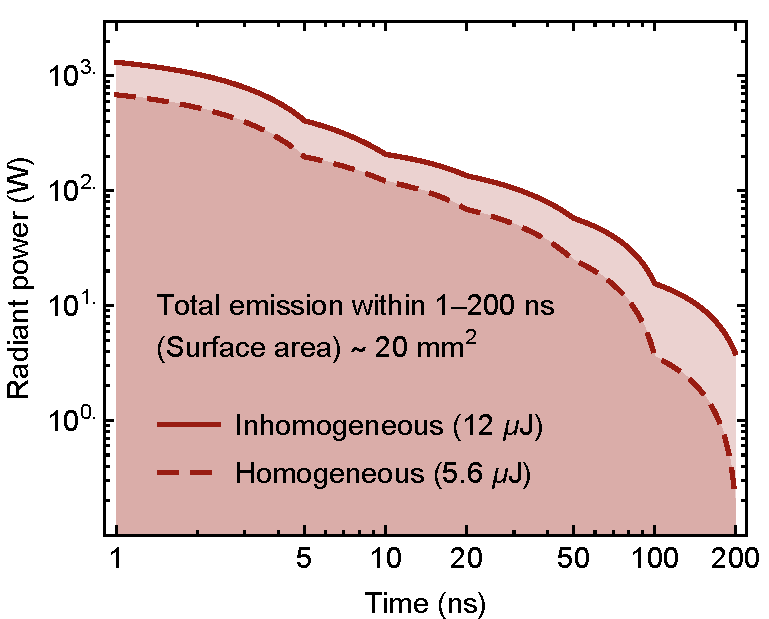
\includegraphics[width=65mm]{figures/ch4/blackbody/loss.pdf}
\caption{Released energy by blackbody radiation from 1 to 200 ns. The radiative loss is a small energy relaxation channel from plasma but gives valuable information about the plasma. There is more than a double difference between the radiation loss in the form of the blackbody continuum for different medium conditions.}
\label{fig:emissionLoss}
\end{figure}

\begin{figure}[ht!]
\centering
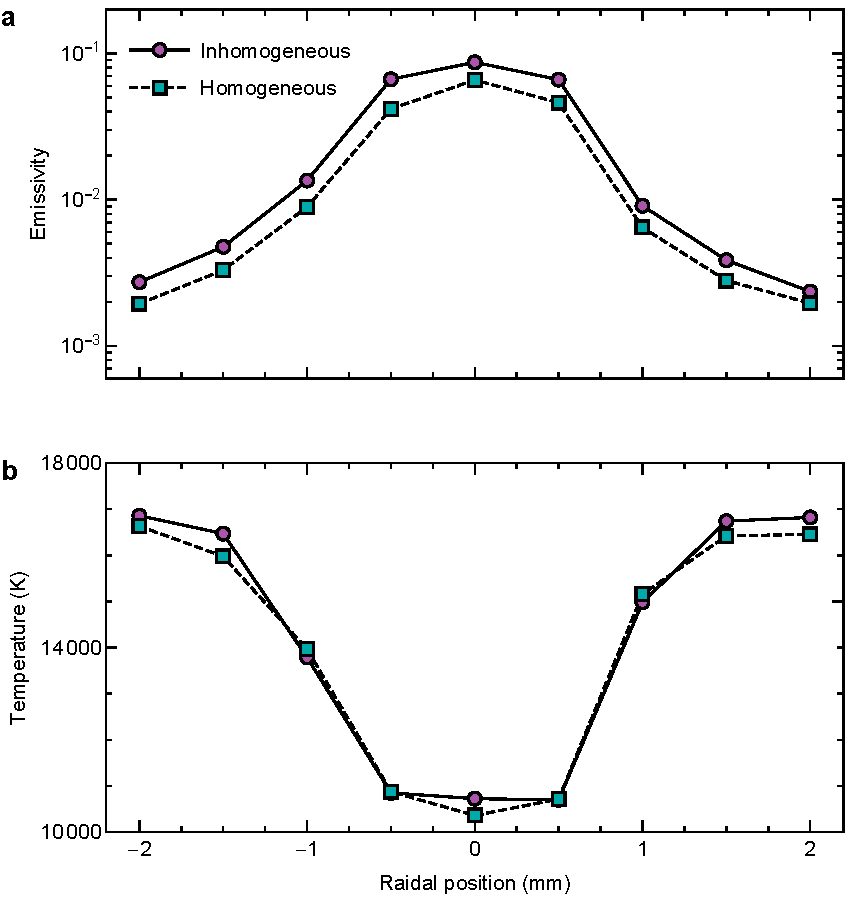
\includegraphics[width=100mm]{figures/ch4/blackbody/radial.pdf}
\caption{The emissivity and temperature of the blackbody by radial position when $t = 0$. The plasma becomes hotter and more dilute at the edge. The plasma bulk is surrounded by the sheath where charge neutrality locally breaks, and a strong electric field is introduced. The charged particles -- mostly electrons are accelerated in a sheath, gathering kinetic energy and collide with other particles to raise the local temperature.}
\label{fig:blackbodyRadial}
\end{figure}

After the generation phase, the bulk expansion of the plasma to the laser upstream finishes, and the plasma radiates intense continuum emission (Fig.\ref{fig:blackbodyFit}). The continuum radiation is well fit with the blackbody radiation model. The spectral irradiance of an ideal blackbody is written as
\begin{equation}
I \left( \lambda ; T \right) = \frac{2 \pi h c^{2}}{\lambda^{5}\left\{\exp \left(h c / \lambda k_{B} T\right)-1\right\}}
\end{equation}
, where the physical constants $h$, $c$, and $k_\text{B}$ are the Planck constant, the speed of light, and the Boltzmann constant, respectively, and $\lambda$ is the wavelength, and $T$ is the blackbody temperature. The emissivity denotes the ratio of the radiation intensity from the plasma to an ideal blackbody, and thus, the closer it is to unity, the closer the plasma to an ideal blackbody. From the beginning, the plasma in the inhomogeneous medium emits a stronger signal (Fig.\ref{fig:blackbodyFit}) and has a higher temperature of about $500 \text{ K}$ (Fig.\ref{fig:blackbodyTemporal}). The gap of the radiation intensity between two different conditions widens further as time goes. Considering the blackbody radiation intensity is proportional to the fourth power of the temperature, the cooler plasma with lower emissivity signifies even weaker radiation. The total blackbody radiation energies within $1 \sim 200 \text{ ns}$ for two conditions are $12 ~\mathrm{\mu} \text{J}$ and $5.6 ~\mathrm{\mu} \text{J}$, respectively (Fig.\ref{fig:emissionLoss}). Note that the radiation from the plasma gives valuable information about the plasma, but a radiative loss is a minor energy relaxation channel, and most of the plasma energy transfers to the heavy particles’ kinetic energy by collision with electrons and released as heat and a shock wave after $100 ~\mathrm{\mu} \text{s}$. The energy transferring timescale from electrons to heavy particles is proportional to the mass ratio between species (Chap.1 in \cite{bellan2008fundamentals}). When the medium is inhomogeneous, the electrons have a higher chance of colliding with even heavier particles, namely, liquid-like fluid packages rather than individual argon atoms or ions. In this respect, the inhomogeneous medium enhances the energy confinement of an SCP.

The radial profile at $t=1 \text{ ns}$ is shown in Fig.\ref{fig:blackbodyRadial}. The plasma gradually becomes hotter and more dilute at the edge. The hotter temperature at the edge of the plasma is due to the acceleration of electrons in the sheath. This phenomenon has been widely observed and reported for relatively low-pressure plasmas \cite{van2012laser}. In our experiment, the plasma becomes dilute at the edge, and the traditional plasma theory applies. Thus, the sheath surrounds the plasma bulk, and the electrons absorb the field energy in the sheath region. As a result, the plasma temperature becomes hotter at the edge.

\begin{figure}[t!]
\centering
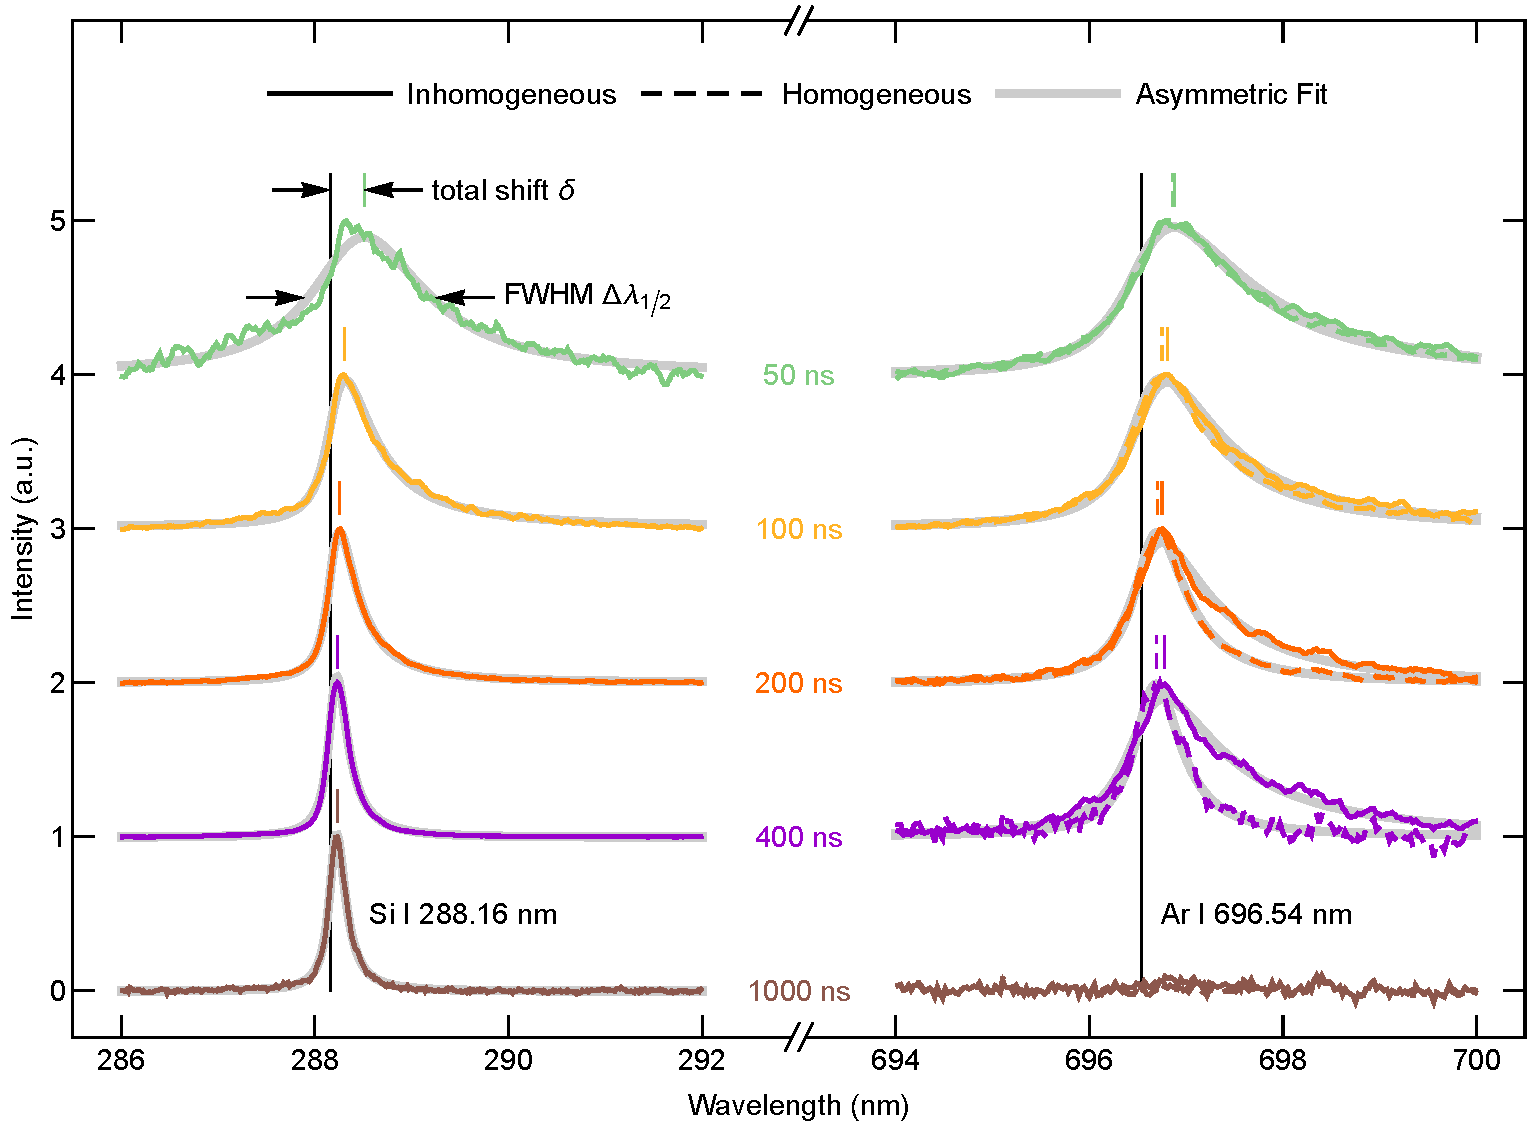
\includegraphics[width=130mm]{figures/ch4/Stark/fit.pdf}
\caption{Asymmetric Stark broadening analysis for Si I ($288.16 \text{ nm}$) and Ar I ($696.54 \text{ nm}$) line emissions. The silicon line emission is only observed for the plasma generated in the inhomogeneous medium, whereas the argon line emission is detected for both conditions. The total broadening and shift decrease as time goes. For the case of $1,000 \text{ ns}$, the argon line emissions disappear for both medium conditions.}
\label{fig:StarkFit}
\end{figure}

\begin{figure}[ht!]
\centering
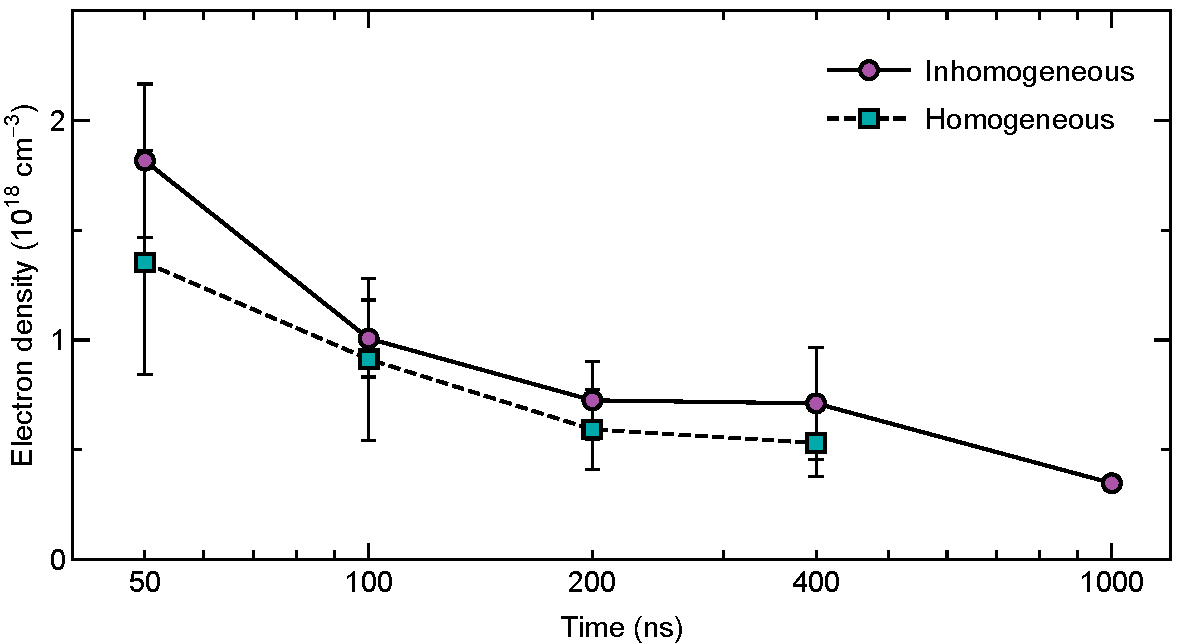
\includegraphics[width=100mm]{figures/ch4/Stark/density.pdf}
\caption{Electron density by time in the extinction phase (after $50 \text{ ns}$). The electron densities of the plasmas in both mediums are of the order of $10^{18} \text{ cm}^{-3}$, with the inhomogeneous condition having a slightly larger value than the other case. The error bars show the standard errors among the results based on the total shifts and widths from the silicon and argon data.}
\label{fig:StarkDensity}
\end{figure}

In the case of the inhomogeneous medium after $50 \text{ ns}$, the silicon line emissions are observed below $300 \text{ nm}$. The Si I line emissions come from the lubricant oil for the compressor. A tiny bit of oil permeates during the compression-expansion process, and the silicon chains provide the nucleation cores for the liquid-like fluid packages. The broadening of line emissions is utilized to measure the electron density (Fig.\ref{fig:StarkFit} and \ref{fig:StarkDensity}) for a later time ($t\geq50 \text{ ns}$) when the plasma becomes diluted, and the blackbody approximation no longer holds.

A large asymmetric Stark broadening is measured on the silicon and argon line emissions. The asymmetry is originated from the influence of the static ions \cite{bengoechea2005asymmetric}. The line profile considering the electron and ion Stark effect together is given by \cite{griem2012spectral, bengoechea2005asymmetric}
\begin{equation}
j_{\alpha} \left( x \right) = \int_{0}^{\infty} \frac{H \left( \beta \right) d \beta}{1+\left( x-\alpha^{4 / 3} \beta^{2} \right)^{2}}
\label{eq:StarkProfile}
\end{equation}
, where $j_\alpha$ is the relative intensity of the profile, $H \left( \beta \right)$ is the microfield strength at neutral atoms, α is ion broadening parameter which is a measure of the ion contribution yielding the asymmetry, and $x$ is the reduced wavelength: $x=\pm \left( \lambda - \lambda_0 - d_e \right) / w_e$ (the sign determines the direction of the asymmetry, and $d_e$ ($w_e$) is the electron shift (width), and $\lambda_0$ is the center wavelength of unperturbed line emission). The asymptotic approximation of the microfield strength is 
\begin{equation}
H \left( \beta \right) \approx K \beta^{-5 / 2} \exp \left( -\Gamma \beta^{1 / 2}-\beta^{-3 / 2} \right)
\label{eq:microfield}
\end{equation}
, where $K$ is an adjustable parameter, and $\Gamma$ is the plasma coupling parameter \cite{potekhin2002electric}. By fitting the measure data using Eq.\ref{eq:StarkProfile} and \ref{eq:microfield}, the total shift and width of the line emissions are obtained, and by comparing them with the values in the literature \cite{konjevic2002experimental}, the electron densities are calculated.

The electron density in the extinction phase is of the order of $10^{18} \text{ cm}^{-3}$, which is comparable to that of the laser plasma on a solid target for a similar time delay \cite{ivkovic2017stark}. Unfortunately, due to the inherent errors in the Stark broadening analysis, it is difficult to figure out the exact electron density for each experimental condition. Nevertheless, we can deduce that the electron density for the inhomogeneous condition is higher than the homogeneous condition by qualitative comparison of the total shifts and widths for the argon line emission.



%----------------------------------------------------------------------------------------------------
\section{Potential lowering}
\label{sec:ch4-4}

\begin{figure}[ht!]
\centering
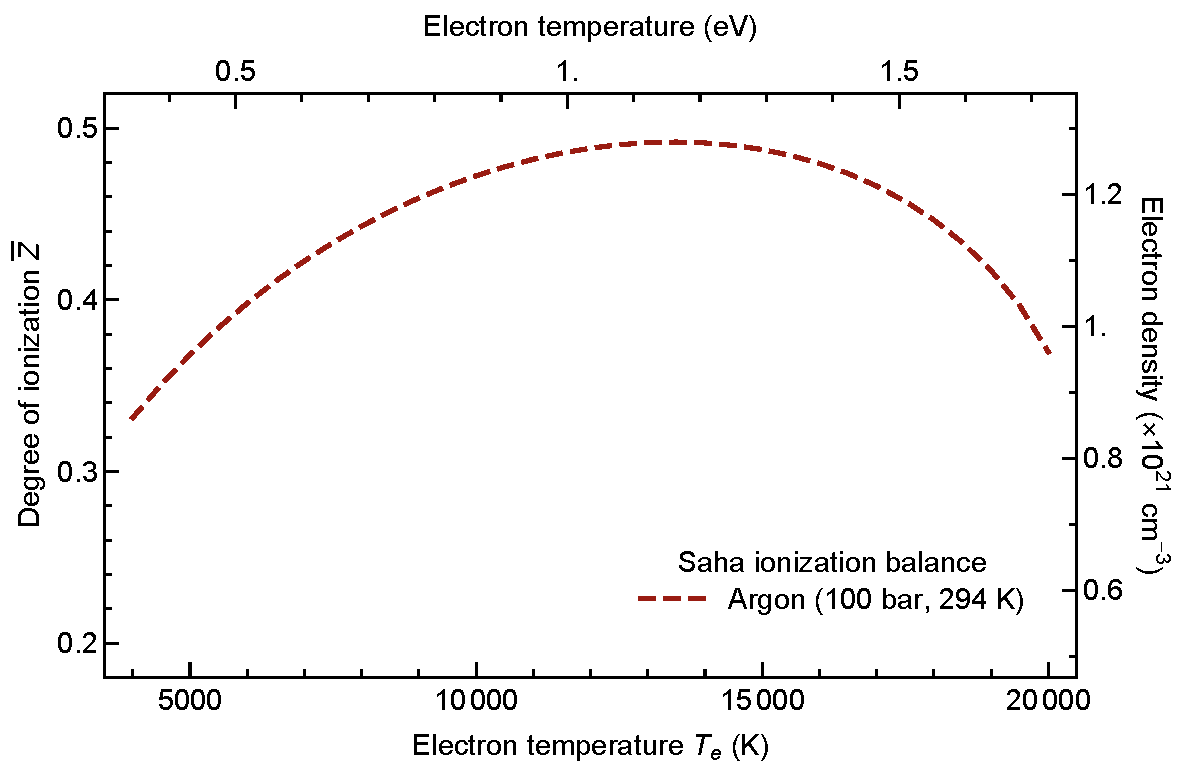
\includegraphics[width=100mm]{figures/ch4/Saha/balance.pdf}
\caption{The solutions for the Eq.\ref{eq:lowering} and \ref{eq:Saha} for argon under $100 \text{ bar}$ and $294 \text{ K}$. The electron density weakly depends on the temperature implying that this analysis is restricted for the order of magnitude estimation.}
\label{fig:SahaBalance}
\end{figure}

Spectral analysis applying SCP theory on the absolute-calibrated blackbody emission provides information about a dense plasma such as the electron density, the degree of ionization, and the amount of potential reduction \cite{bataller2014blackbody}. However, the overall error in the spectroscopic measurement system is about $15\%$, which limits the analysis regarding the plasma opacity. In order to circumvent this issue and find a relevant electron density, we solve two coupled equations – the ionization energy lowering and the corrected Saha’s equation. In a dense plasma, due to the Debye screening, the amount of the ionization potential reduction follows Eq.\ref{eq:lowering}. Saha’s equation is corrected under the presence of the potential reduction by 
\begin{equation}
\frac{x_{m+1} x_{e}}{x_{m}}=\frac{2}{n_{0}} \frac{u_{m+1}}{u_{m}} \cdot\left(\frac{m_{e} k_{B} T}{2 \pi \hbar^{2}}\right)^{3 / 2} \exp \left(-\frac{\chi_{m}-\Delta \chi}{k_{B} T}\right)
\end{equation}
, where $x_m$ ($x_e$), $u_m$, and $χ_m$ are the ion(electron) concentration, electronic partition function, and ionization potential for the $m\text{-th}$ ion, respectively \cite{bataller2014blackbody, griem1962high, zel2002physics} and $n_0$ is the atomic number density of the supercritical fluid, $m_e$ is the electron mass, and $\hbar$ is the reduced Planck constant. Considering the first ionization of argon ($m=1$), $x_{m+1}=\bar{Z}$, $x_m=1-\bar{Z}$, $x_e=\bar{Z}$, and $\chi_m=\chi_0$ (i.e., ionization potential for a neutral atom) the equation is modified as 
\begin{equation}
\frac{\bar{Z}^{2}}{1-\bar{Z}}=\frac{2}{n_{0}} \frac{u_{1}}{u_{0}} \cdot\left(\frac{m_{e} k_{B} T}{2 \pi \hbar^{2}}\right)^{3 / 2} \exp \left(-\frac{\chi_{0}-\Delta \chi}{k_{B} T}\right)
\label{eq:Saha}
\end{equation}
Solving the Eq.\ref{eq:lowering} and \ref{eq:Saha} simultaneously when the temperature is $11,000 \text{ K}$ using the known values: $u_0=1$, $u_1=5.66$, $\chi_0 \approx 15.8 \text{ eV}$ \cite{kramida2020nist}, and $n_0 = 2.6 \times 10^{21}  \text{ cm}^{-3}$ for the argon at $300 \text{ K}$ and $100 \text{ bar}$ \cite{linstorm2020nist} yields the effective degree of ionization $\bar{Z} \approx 0.5$ and potential lowering $\Delta \chi \approx 12.7 \text{ eV}$. The corresponding electron density $n_e \approx 1.3 \times 10^{21} \text{ cm}^{-3}$ and the plasma coupling parameter $\Gamma \approx 1.6$. This analysis only provides the order of magnitude of the values (Fig.\ref{fig:SahaBalance}).




%----------------------------------------------------------------------------------------------------
\section{Medium effect on plasma}
\label{sec:ch4-5}

We observe that the inhomogeneous supercritical fluid with the liquid-like mesoscopic fluid packages enhances the charge and energy confinement of an SCP generated by a nanosecond pulse laser. When the medium is inhomogeneous, more laser energy is coupled throughout the generating phase. Once an SCP is achieved, electrons are attached to the mesoscopic particles, and the recombination with ions in the later time is localized near the particles. Moreover, the energy relaxation of the electrons becomes slower when they are surrounded by the heavier particles rather than the individual atoms or ions. The SCP generated in such an inhomogeneous medium will help us extend our current understanding of the transport properties in the SCPs even further to what extent the anomalous medium affects.

Additionally, the finding that the medium's inhomogeneity may efficiently restrict the energy and charge of the plasma has a wide range of applications. Plasma, for example, is critical in the process of synthesizing different chemicals that are hard to synthesis in daily circumstances owing to plasma particles' high activity, which allows them to readily overcome the energy barrier of chemical processes. Furthermore, according to the properties of the medium, such as high diffusivity and low viscosity, the plasma produced in the supercritical fluid may have even more significant activity than normal plasma. Supercritical fluid plasma has a broad range of uses from this perspective. The depth of application in terms of energy efficiency will be improved if a supercritical fluid with inhomogeneity is employed as a discharge medium, as shown in this research. Finally, this research will help to extend the use of supercritical fluid plasma while also contributing to the study of strongly coupled plasma.


